\chapter{实物可视化界面UI设计}
\label{cha:UI}

本部分代码详见\url{https://github.com/TingliangZhang/Misaka-Jupyter}。

\section{实物可视化界面}

在动态迭代可视化模式下,工作平面视为一个二维坐标系,每一个小车代表一个机组节点,小车在坐标系中纵轴位置代表各自当前出力,随着迭代进行变化,同时隐性地仿真了通信过程,进行去中心化的自治优化,当节点数(新加入或撤出)或任意节点数据变化系统会重新开始动态迭代。物理场景和算法的映射关系如表~\ref{tab:Real-Unreal}。表现形式不一定是位置,也可能是颜色,坐标系也可能会是三维的。

% Please add the following required packages to your document preamble:
% \usepackage{booktabs}
\begin{table}[htbp]
    \centering
    \begin{tabular}{@{}ll@{}}
    \toprule
    物理场景          & 算法                   \\ \midrule
    桌面            & 二维坐标系                \\
    前后            & 纵轴——电价指数(可能会经过一系列变换) \\
    左右            & 横轴——节点数(均匀分布)        \\
    小车            & 通信节点(拓扑中的点)          \\
    摆放小车          & 设定初始节点数和各节点初始值       \\
    小车运动          & 电价指数改变               \\
    停止在Y坐标相同的一条线上 & 迭代完成,各节点达成共识         \\
    移除小车          & 断开一个节点               \\
    放入小车          & 新增一个节点后自动重新开始迭代      \\ \bottomrule
    \end{tabular}
    \caption{物理场景和算法的映射关系}
    \label{tab:Real-Unreal}
\end{table}

\section{实物可视化界面DEMO}

初始DEMO UI为用PC通过XBee指定节点ID发送Move距离信息,节点收到后即开始运动相应距离,此过程中需要对Step和实际距离进行标定。首次标定得到两电机相反方向转动1000steps约为前进15cm,此时stepsPerRevolution = 200,即steps * stepsPerRevolution = 1000。如图~\ref{fig:MeasureSteps}

\begin{figure}[htbp]
    \centering
    \includegraphics[width=\columnwidth]{MeasureSteps.jpg}
    \caption{对Step和实际距离进行标定}
    \label{fig:MeasureSteps}
\end{figure}

采用的数据参照~\ref{sec:Illustration}小节中的数据设计,考虑到场地有限(宿舍桌面大小),占用纵轴区间长度3对应45cm的可用桌面,比例0.5cm对应1单位,考虑到精度问题,如表~\ref{tab:UIDemoDesign},只取0,1,2,3,8,9,10,13这几组变化较大的数据,如表~\ref{tab:UIDemoDesignSelection}。

\begin{table}[htbp]
    \centering
    \begin{tabular}{|l|l|l|l|l|l|l|l|l|}
    \hline
    \diagbox{迭代次数}{$Y_{i,j}$}{位移} %添加斜线表头
       & 1  & 2  & 3  & 4   & d1 & d2 & d3  & d4  \\ \hline
    0  & 0  & 0  & 0  & 0   &    &    &     &     \\ \hline
    1  & 30 & 60 & 90 & 0   & 30 & 60 & 90  & 0   \\ \hline
    2  & 45 & 75 & 60 & 0   & 15 & 15 & -30 & 0   \\ \hline
    3  & 60 & 68 & 53 & 0   & 15 & -8 & -8  & 0   \\ \hline
    4  & 64 & 60 & 56 & 0   & 4  & -8 & 4   & 0   \\ \hline
    5  & 62 & 58 & 60 & 0   & -2 & -2 & 4   & 0   \\ \hline
    6  & 60 & 59 & 61 & 0   & -2 & 1  & 1   & 0   \\ \hline
    7  & 60 & 60 & 60 & 0   & 0  & 1  & 0   & 0   \\ \hline
    8  & 60 & 60 & 60 & 120 & 0  & 0  & 0   & 120 \\ \hline
    9  & 60 & 60 & 80 & 90  & 0  & 0  & 20  & -30 \\ \hline
    10 & 60 & 70 & 77 & 75  & 0  & 10 & -3  & -15 \\ \hline
    11 & 65 & 73 & 71 & 73  & 5  & 3  & -6  & -2  \\ \hline
    12 & 69 & 72 & 69 & 73  & 4  & -1 & -1  & 0   \\ \hline
    13 & 71 & 71 & 71 & 71  & 2  & -1 & 2   & -2  \\ \hline
    \end{tabular}
    \caption{节点位移比对}
    \label{tab:UIDemoDesign}
\end{table}

\begin{table}[htbp]
    \centering
    \begin{tabular}{|l|l|l|l|l|l|l|l|l|}
    \hline
    \diagbox{迭代次数}{$Y_{i,j}$}{位移} %添加斜线表头
      & 1  & 2  & 3  & 4   & d1 & d2 & d3  & d4  \\ \hline
    0 & 30 & 30 & 30 & 120 &    &    &     &     \\ \hline
    1 & 30 & 60 & 90 & 120 & 0  & 30 & 60  & 0   \\ \hline
    2 & 45 & 75 & 60 & 120 & 15 & 15 & -30 & 0   \\ \hline
    3 & 60 & 68 & 53 & 120 & 15 & -8 & -8  & 0   \\ \hline
    4 & 60 & 60 & 60 & 120 & 0  & -8 & 8   & 0   \\ \hline
    5 & 60 & 60 & 80 & 90  & 0  & 0  & 20  & -30 \\ \hline
    6 & 60 & 70 & 77 & 75  & 0  & 10 & -3  & -15 \\ \hline
    7 & 71 & 71 & 71 & 71  & 11 & 1  & -6  & -4  \\ \hline
    \end{tabular}
    \caption{节点位移选取}
    \label{tab:UIDemoDesignSelection}
\end{table}

对ForwardUnits进行1/6校准到单位位移,对Delay进行1/16校准到1ms。

但是还有一个因素未纳入考虑,小车移动需要时间。要想让他们同时进行运动,还要计算各小车运动的时间。

我们知道,1step对应放缩后的1ms,ForwardUnits(30) 对应的时间为1s,由此设计开始运动时间间隔为3s。减去相应的移动时间即为两次移动中间应当delay的时间。

此Demo小车端代码详见附录~\ref{sec:MisakaCarV1}。

\section{JupyterLab环境配置}

本节代码详见附录~\ref{sec:JupyterLabUI-Code}。

JupyterLab安装参考TUNA的pypi 镜像使用帮助\footnote{\url{https://mirrors.tuna.tsinghua.edu.cn/help/pypi/}},升级 pip 到最新的版本 (>=10.0.0) 后进行配置:

\begin{tcolorbox}
    pip install pip -U \\
    pip config set global.index-url https://pypi.tuna.tsinghua.edu.cn/simple \\
    pip install jupyterlab
\end{tcolorbox}

在CMD或者Powershell中使用以下命令启动jupyter lab:

\begin{tcolorbox}
    jupyter lab
\end{tcolorbox}

ipywidgets\footnote{\url{https://github.com/jupyter-widgets/ipywidgets}}可以使用pip安装,注意安装前关闭Jupyter Lab再安装!

\begin{tcolorbox}
    pip install ipywidgets \\
    jupyter nbextension enable --py --sys-prefix widgetsnbextension  (can be skipped for notebook version 5.3 and above)
\end{tcolorbox}

cookie cutter\footnote{\url{https://github.com/jupyter-widgets/widget-ts-cookiecutter}}是一个很流行的示例项目,可供参考。

流行的widget库包括bqplot\footnote{\url{https://github.com/bloomberg/bqplot}}、pythreejs\footnote{\url{https://github.com/jovyan/pythreejs}}和ipyleaflet\footnote{\url{https://github.com/ellisonbg/ipyleaflet}}等。

Plotly\footnote{\url{https://plot.ly/python/getting-started/}}是一个ipywidgets,用于构建交互式图表。

可以使用pip安装:

\begin{tcolorbox}
    pip install plotly
\end{tcolorbox}

Dependence的安装:

\begin{tcolorbox}
    pip install jupyterlab "ipywidgets"
\end{tcolorbox}

之后需要Enable Plotly并设置环境变量,执行以下命令:

\begin{minted}[breaklines]{python}
    # Avoid "JavaScript heap out of memory" errors during extension installation
    # (OS X/Linux)
    export NODE_OPTIONS=--max-old-space-size=4096
    # (Windows)
    set NODE_OPTIONS=--max-old-space-size=4096

    # Jupyter widgets extension
    jupyter labextension install @jupyter-widgets/jupyterlab-manager --no-build

    # jupyterlab renderer support
    jupyter labextension install jupyterlab-plotly --no-build

    # FigureWidget support
    jupyter labextension install plotlywidget --no-build

    # Build extensions (must be done to activate extensions since --no-build is used above)
    jupyter lab build

    # Unset NODE_OPTIONS environment variable
    # (OS X/Linux)
    unset NODE_OPTIONS
    # (Windows)
    set NODE_OPTIONS=
\end{minted}

用以下代码来测试Plotly是否正确安装:

\begin{minted}[breaklines]{python}
    import plotly.graph_objects as go
    fig = go.Figure(data=go.Bar(y=[2, 3, 1]))
    fig.show()
\end{minted}

\section{演示系统UI}

UI基于Jupyter Lab编写网页端的实时可视化界面。

以下代码的作用是产生一个可通过拖动滑块来交互的直方图界面:

\begin{minted}[breaklines,linenos,python3]{python}
    import plotly.graph_objects as go
    from __future__ import print_function
    from ipywidgets import interact, interactive, fixed, interact_manual
    import ipywidgets as widgets
    from ipywidgets import Button, Layout

    def f(a,b,c,d):
        fig = go.Figure(data=go.Bar(y=[a, b, c, d]))
        fig.show()
        global Input
        Input = [0,0,0,0]
        Input[0]=a
        Input[1]=b
        Input[2]=c
        Input[3]=d
        for i in range(0,4):
            print(Input[i])
        # 在这插入XBee代码
        XbeeTx(Input)
        
    def XbeeTx(Input):
        for i in range(0,4):
            print(Input[i])    

    def XbeeTxRun(RUNorNOT):
        print('Running')           
            
            
    I = [0,0,0,0]

    for i in range(0,4):
        I[i] = widgets.FloatSlider(min=0, max=1e3, step=1)

    ui = widgets.VBox([I[0], I[1], I[2], I[3] ])
    # ui = widgets.HBox([I[0], I[1], I[2], I[3] ])

    out = widgets.interactive_output(f, {'a': I[0], 'b': I[1], 'c': I[2], 'd': I[3] } )

    b1 = Button(description='Run')
    b1.style.button_color = 'lightgreen'
    b1.on_click (XbeeTxRun)


    display(ui, out, b1)
\end{minted}

运行效果如图~\ref{fig:Plotly-0}

\begin{figure}[htbp]
    \centering
    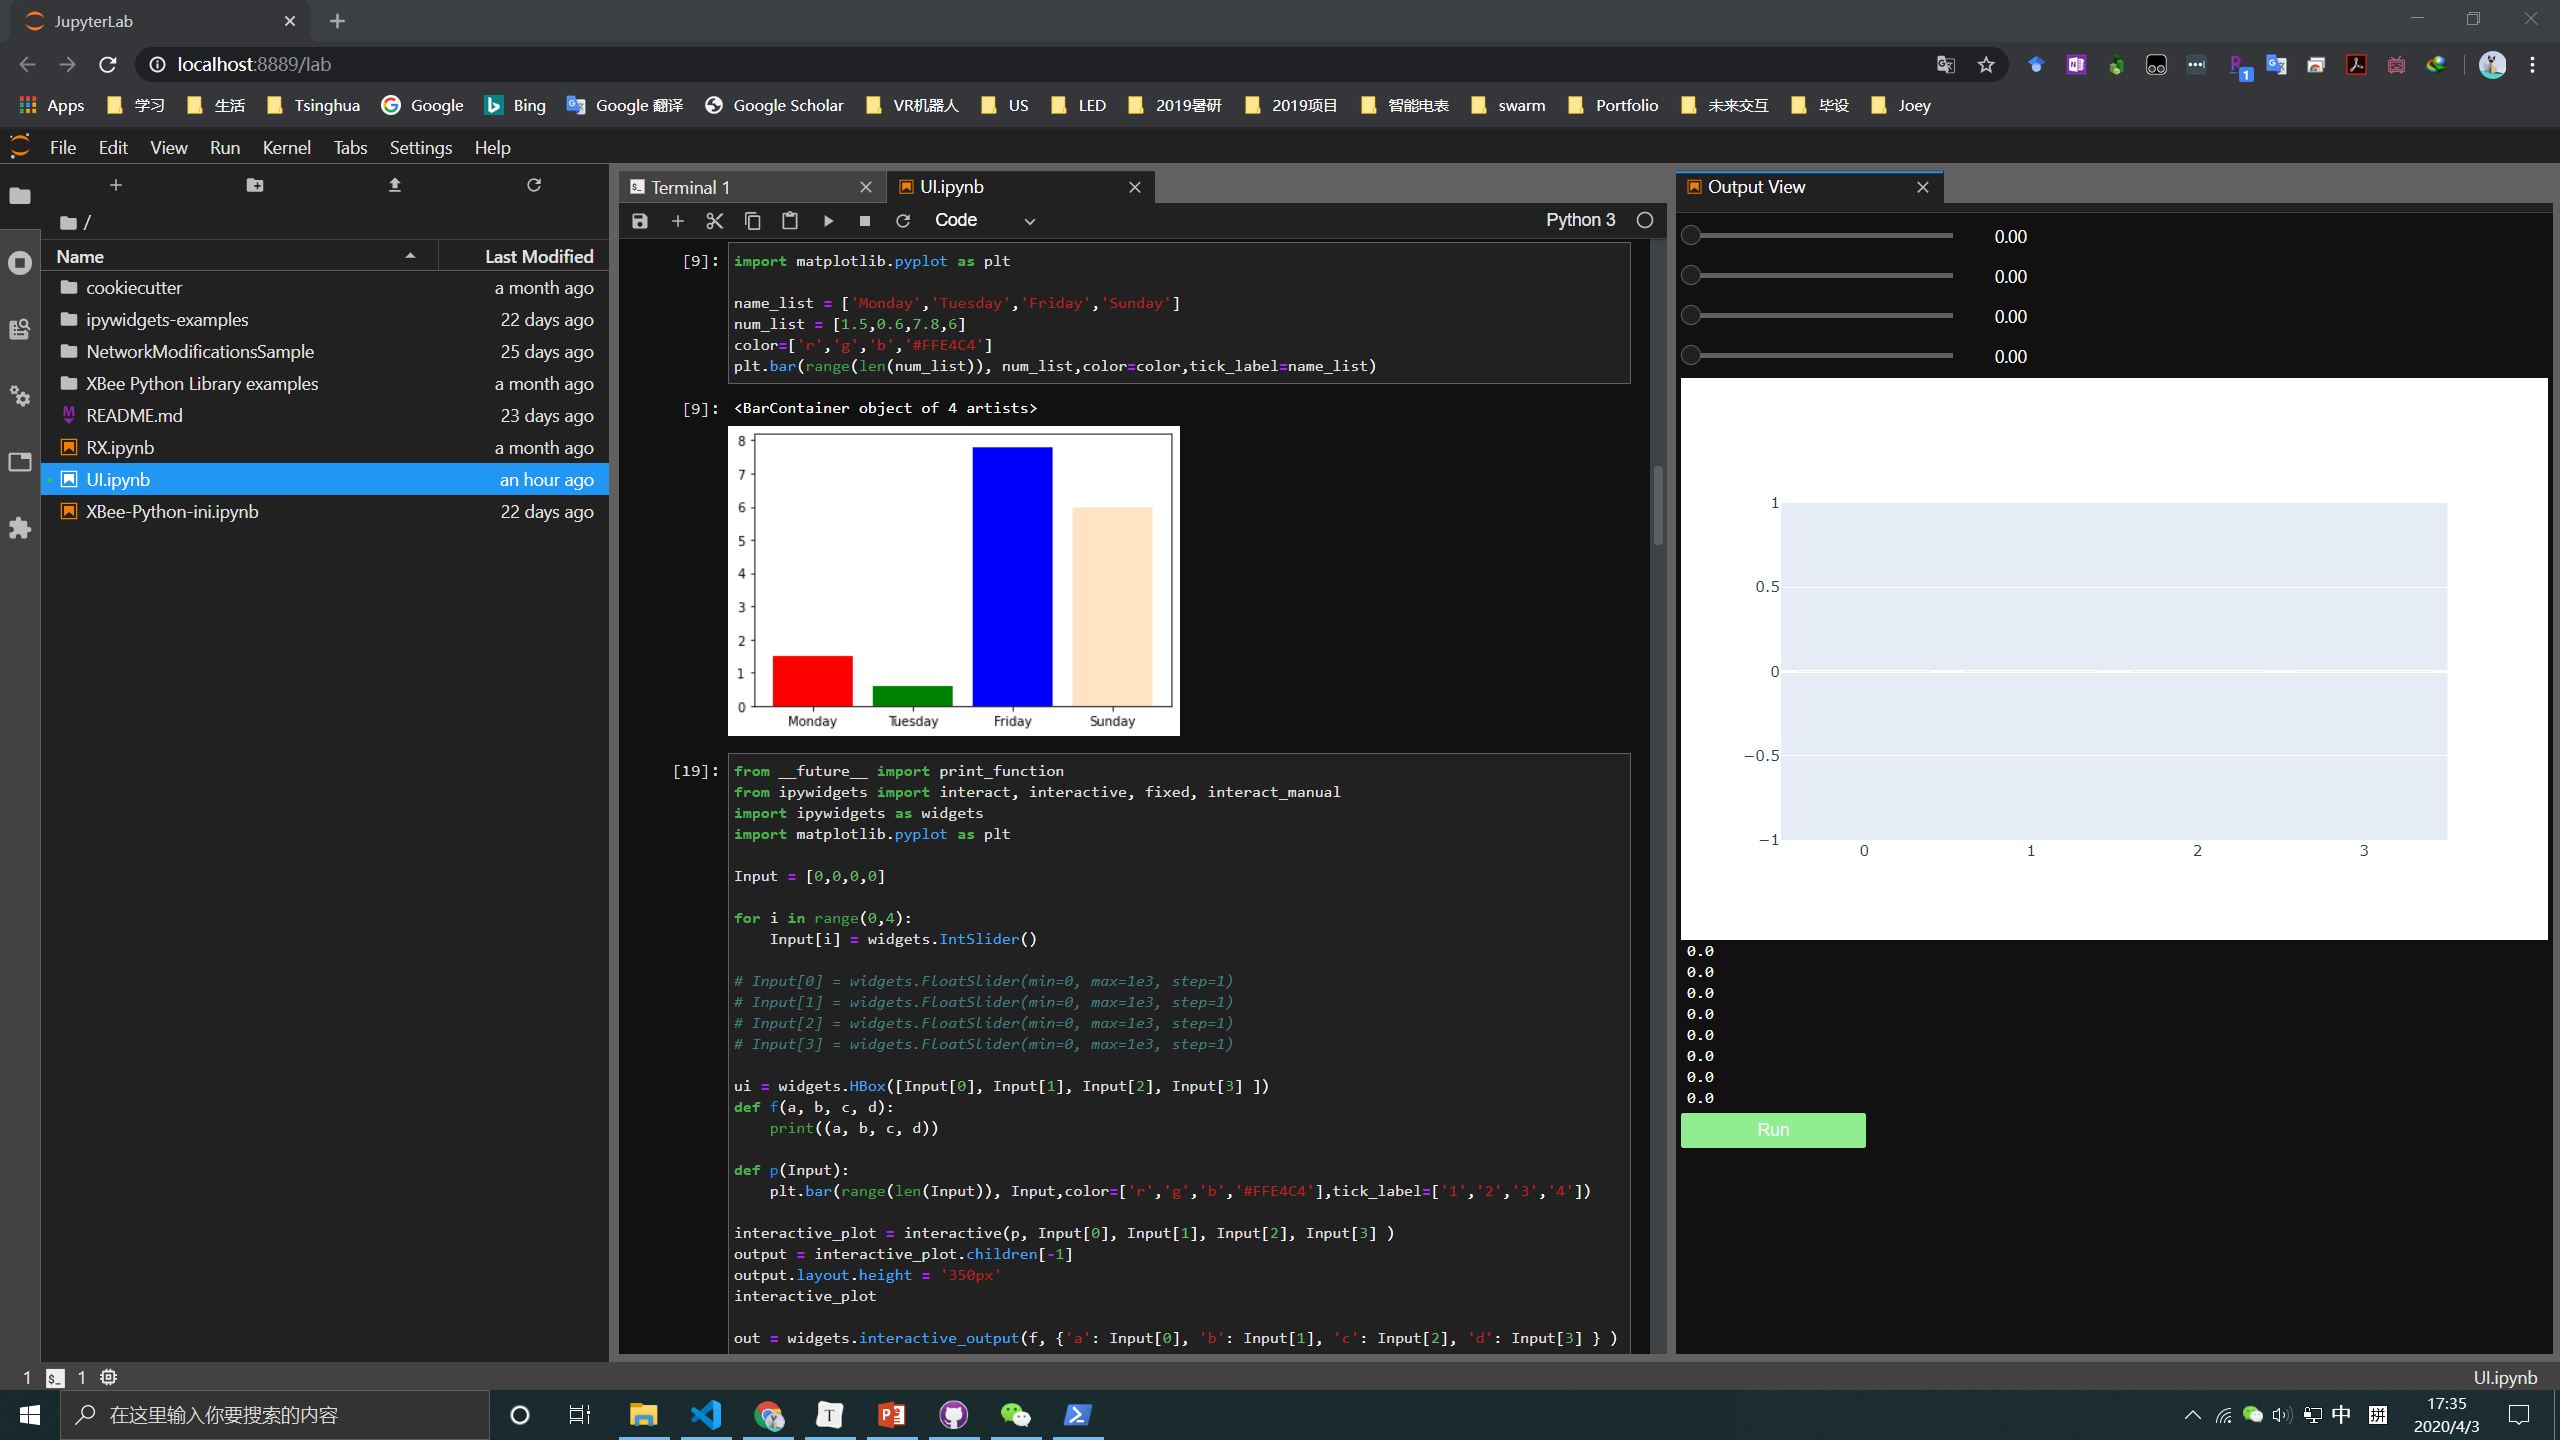
\includegraphics[width=\columnwidth]{Plotly-0.png}
    \caption{Plotly界面交互效果-初始}
    \label{fig:Plotly-0}
\end{figure}

拖动滑块将改变widgets.FloatSlider函数内形参的量,并在函数f中将I这一FloatSlider型变量传递到全局变量Input上(浮点型),显示在下方,效果如图~\ref{fig:Plotly}

\begin{figure}[htbp]
    \centering
    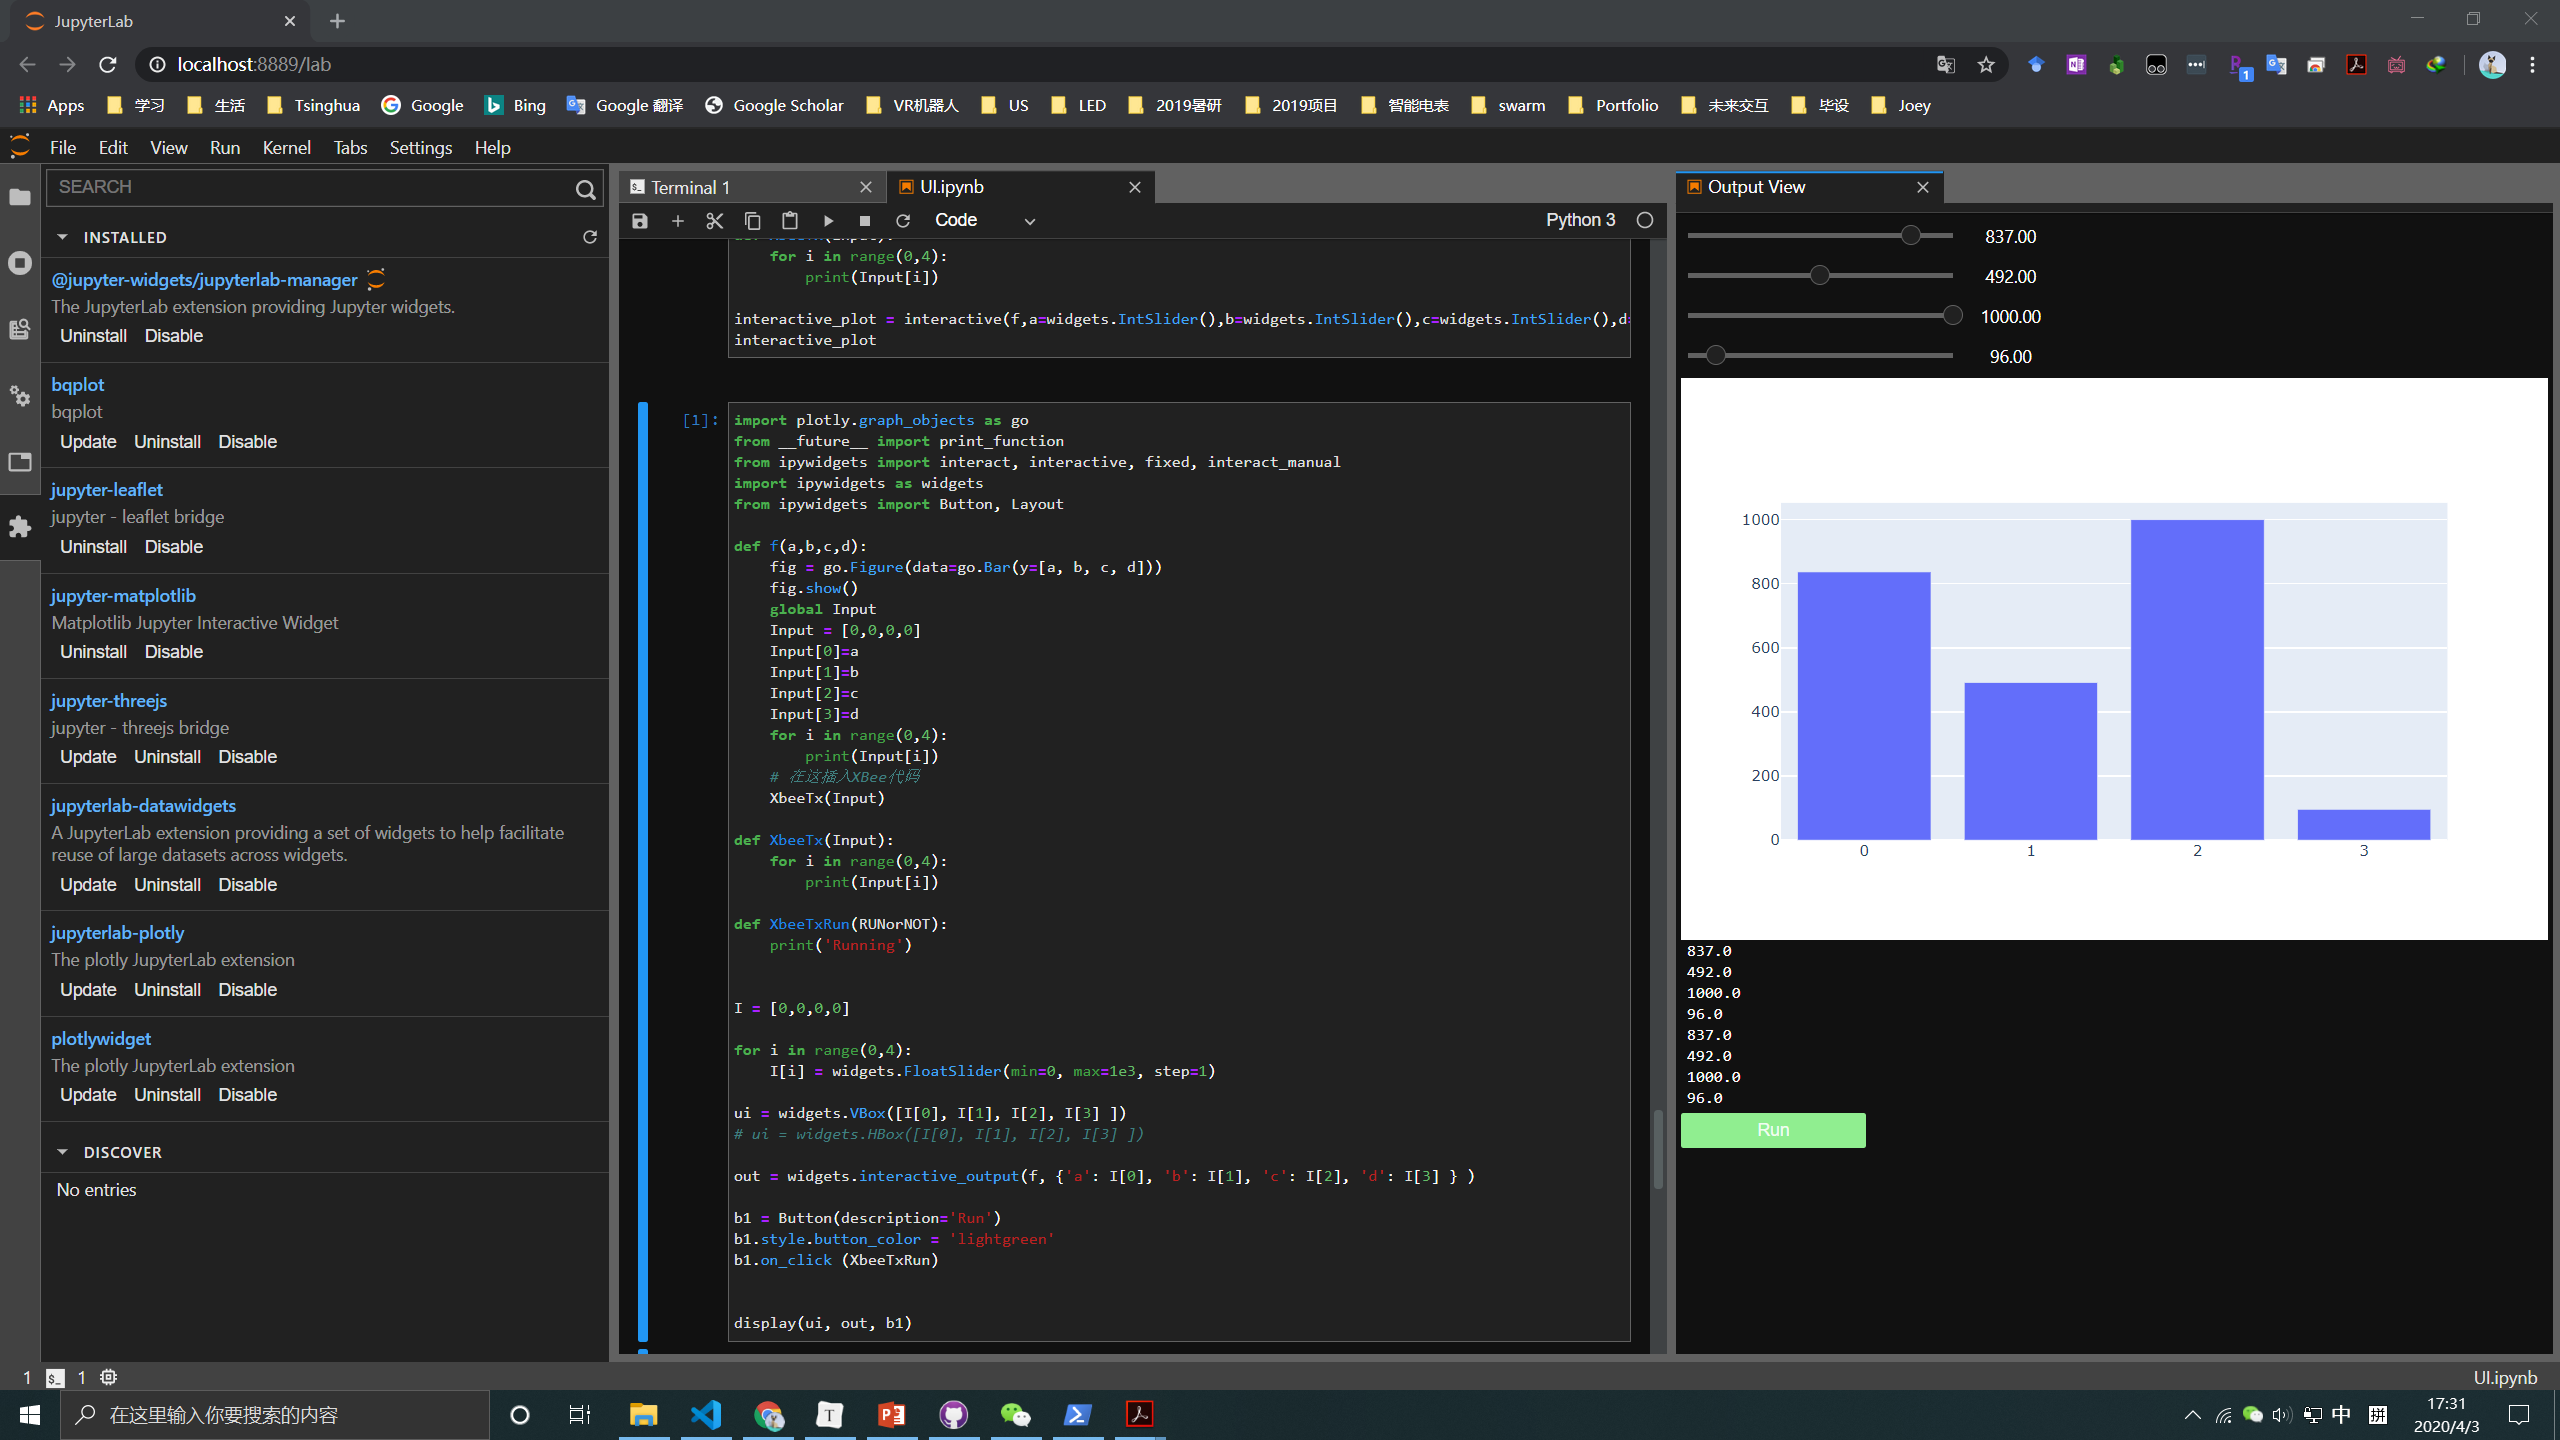
\includegraphics[width=\columnwidth]{Plotly.png}
    \caption{Plotly界面交互效果-拖动}
    \label{fig:Plotly}
\end{figure}

点击Run后,显示的变为小车的实时位置(Y轴),移动平台开始运动,函数开始迭代,逐渐收敛。运行效果如图~\ref{fig:Plotly-1}

\begin{figure}[htbp]
    \centering
    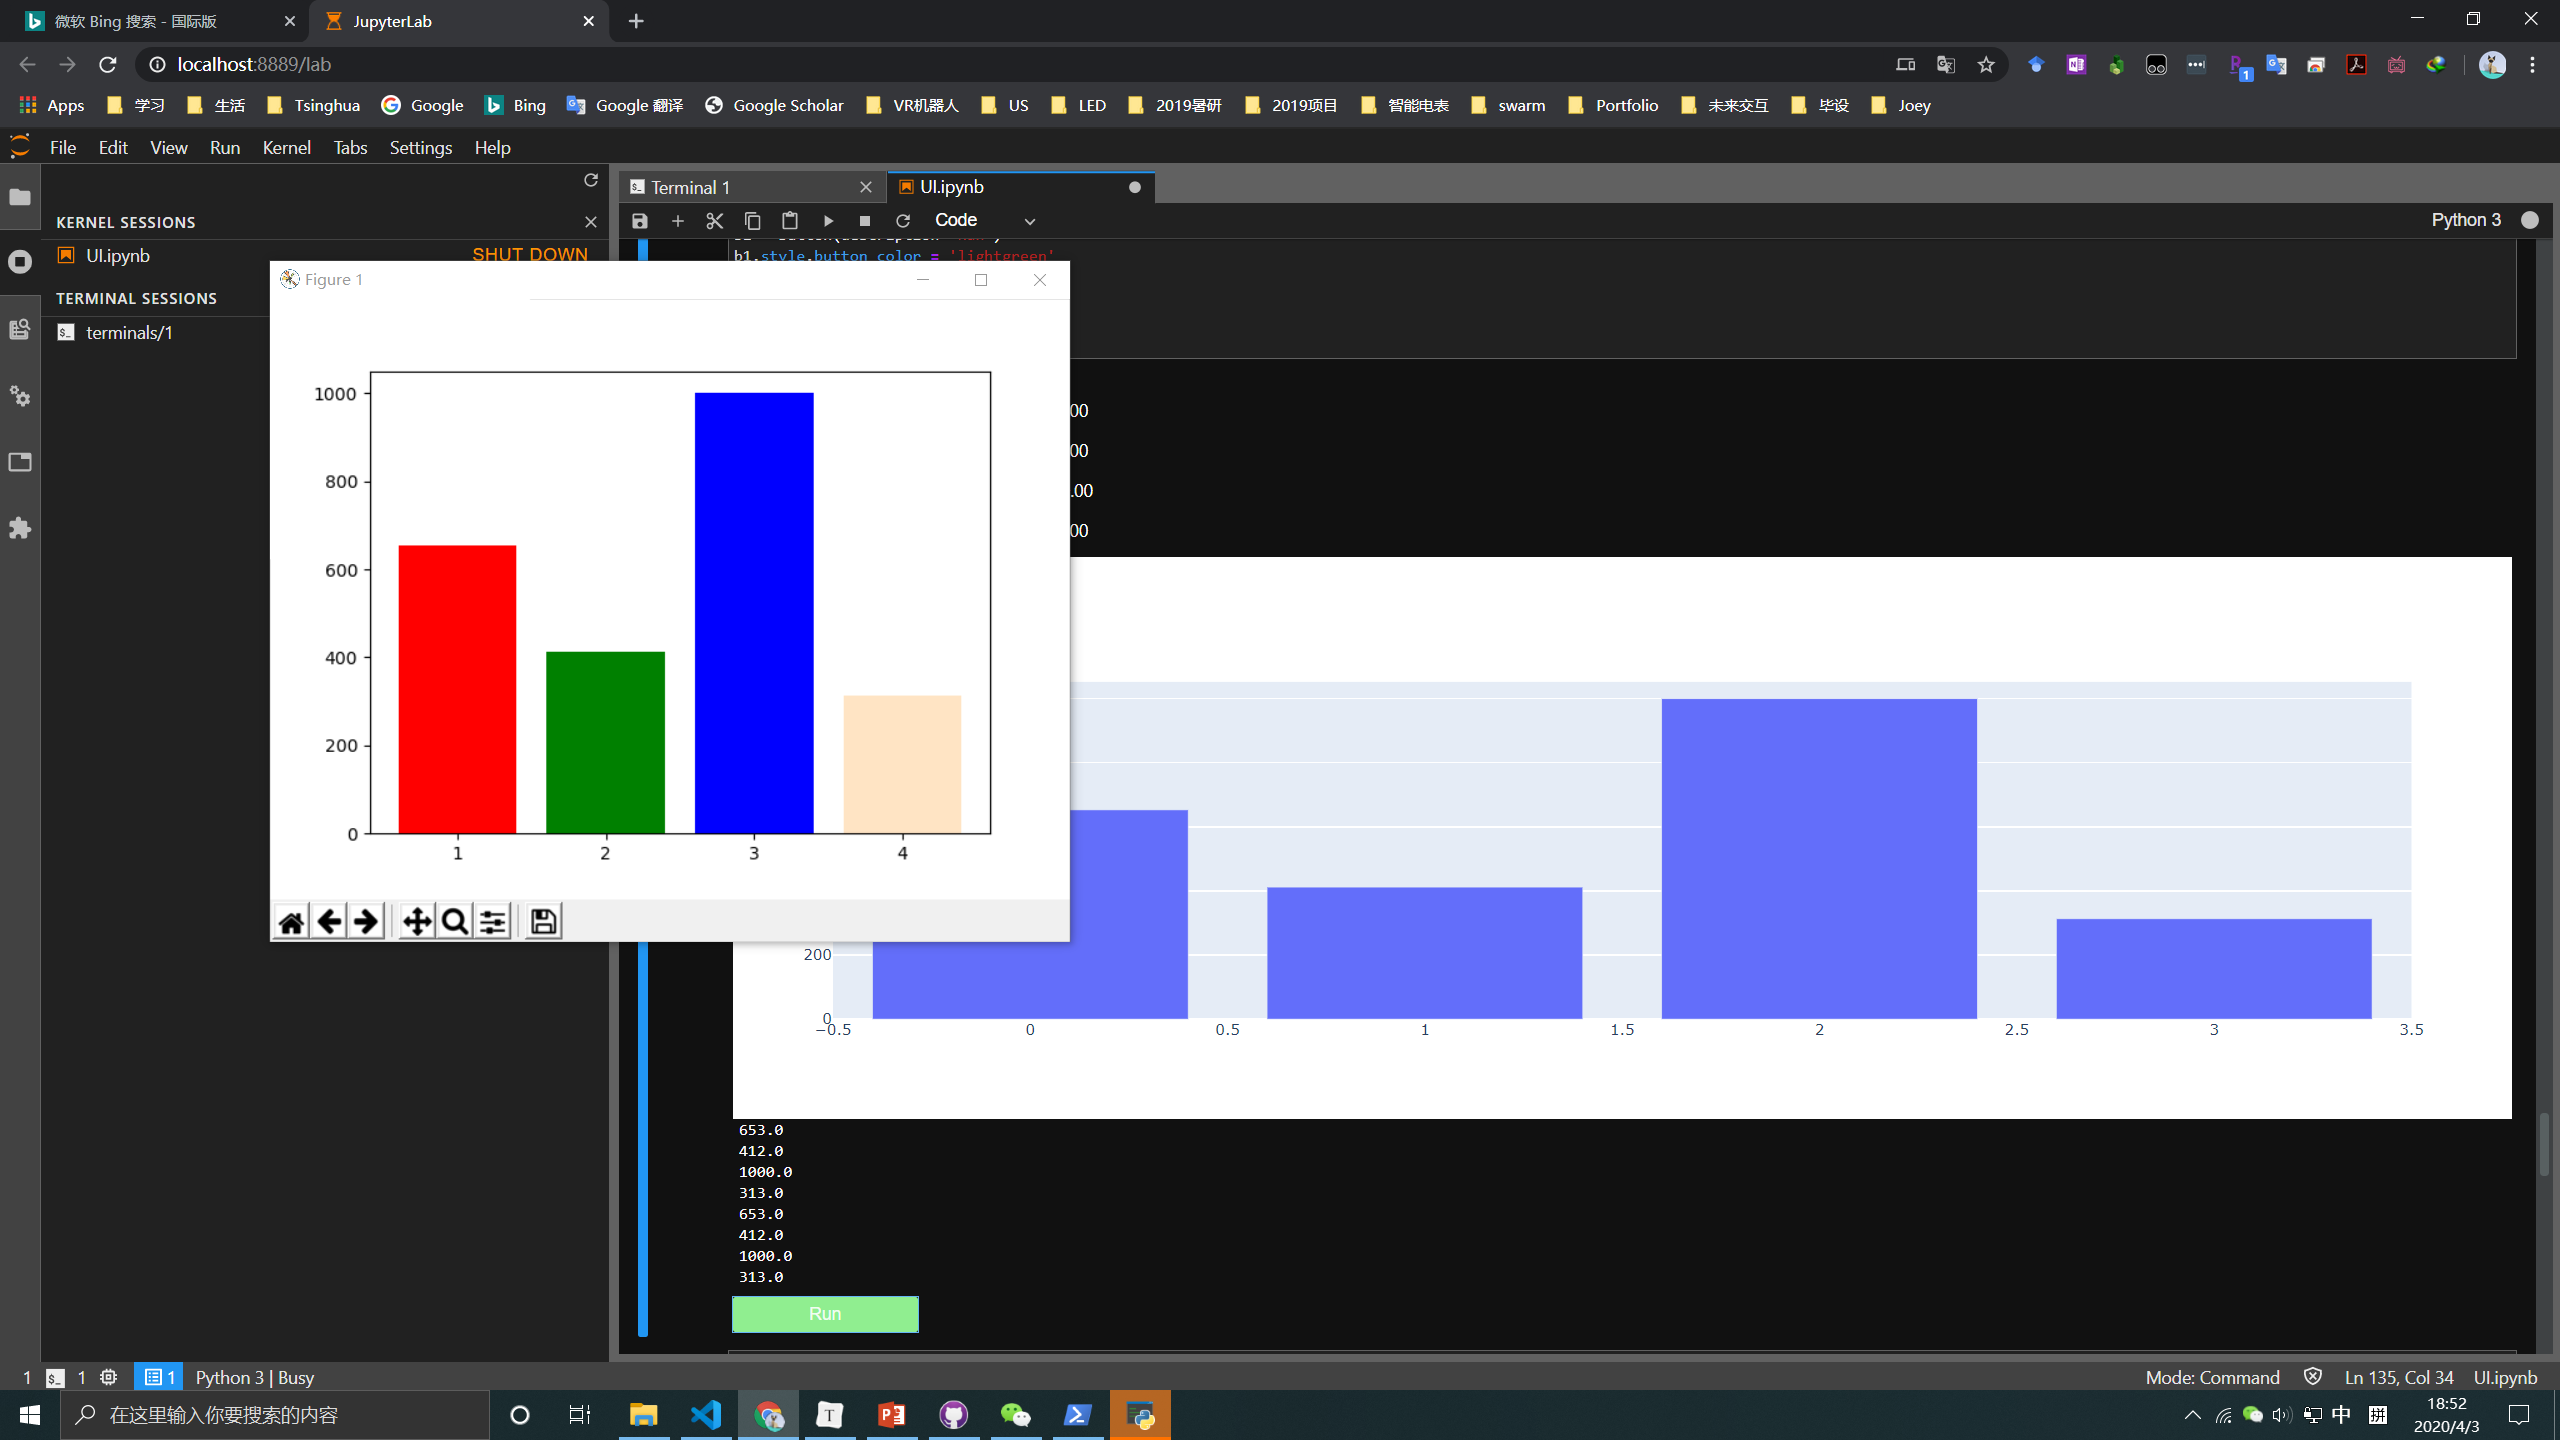
\includegraphics[width=\columnwidth]{Plotly-1.png}
    \caption{Plotly界面交互效果-点击Run后}
    \label{fig:Plotly-1}
\end{figure}

为了演示效果,两次迭代之间加入了1s的延迟。